%! Author = wolfram_e_laube
%! Date = 17.04.24

\item[(a)]
The discrete time signals are plotted with the appropriate commands to display the nature of the signals.
For the signals $x_{1}[n]$ and $x_{2}[n]$, the stem command is used to emphasize their discrete nature,
and for the longer signals $x_{3}[n]$ and $x_{4}[n]$, the plot command is utilized.

\begin{verbatim}
import numpy as np
import matplotlib.pyplot as plt

n1 = np.arange(-5, 11)  # Range for x1[n] and x2[n]
n2 = np.arange(0, 257)  # Range for x3[n] and x4[n]

# Discrete time signals
x1 = -4 * (n1 == -3) + 4 * (n1 == 0) - (n1 == 3) + 2 * (n1 == 7)
x2 = np.exp(-0.31 * n1)
x3 = 3 * np.sin(2 * np.pi * 3.5/64 * n2)
x4 = -np.cos(9/64 * n2)

# Plotting
plt.figure(figsize=(14, 10))

plt.subplot(2, 2, 1)
plt.stem(n1, x1, linefmt='C0-', markerfmt='C0o', basefmt=" ")
plt.title('Signal x1[n]')

plt.subplot(2, 2, 2)
plt.stem(n1, x2, linefmt='C1-', markerfmt='C1o', basefmt=" ")
plt.title('Signal x2[n]')

plt.subplot(2, 2, 3)
plt.plot(n2, x3)
plt.title('Signal x3[n]')

plt.subplot(2, 2, 4)
plt.plot(n2, x4)
plt.title('Signal x4[n]')

plt.tight_layout()
plt.show()
\end{verbatim}

\begin{figure}[h]
\centering
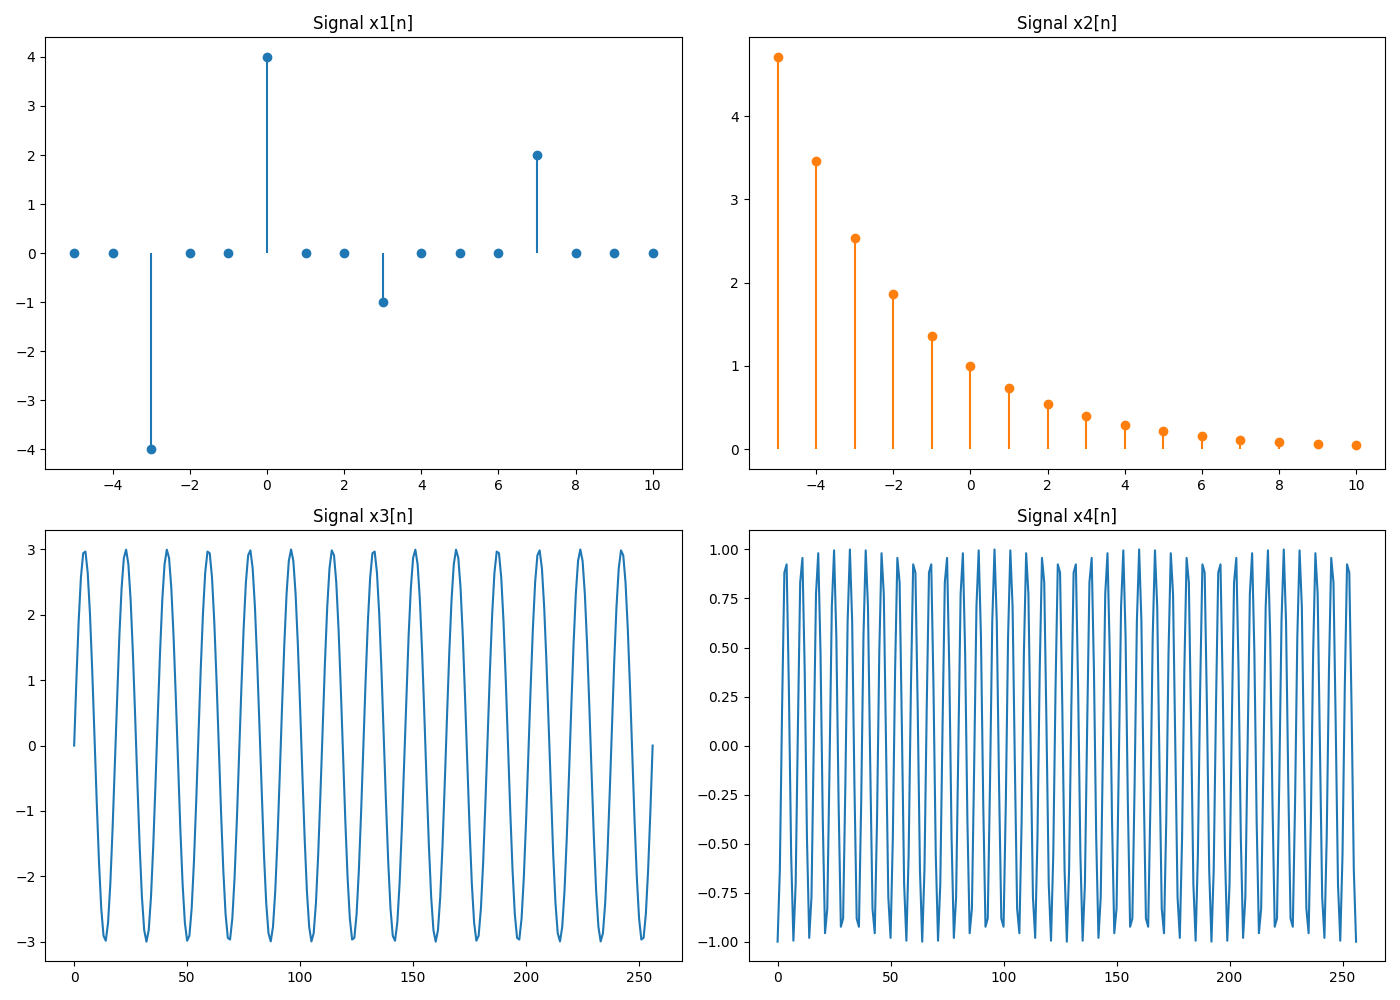
\includegraphics[width=\textwidth]{fig/ex1_a_plot}
\caption{Signals stem/plot}
\label{fig:ex1_a_plot}
\end{figure}


